\documentclass[crop,tikz]{standalone}
\usepackage{graphicx}
\begin{document}
\begin{tikzpicture}
  \node[inner sep=0pt, anchor=south west] (mult) at (0,0)
    {\includegraphics{fig4_data.pdf}};

  \node[inner sep=0pt, anchor=south west] at (1.82,7.75) 
{  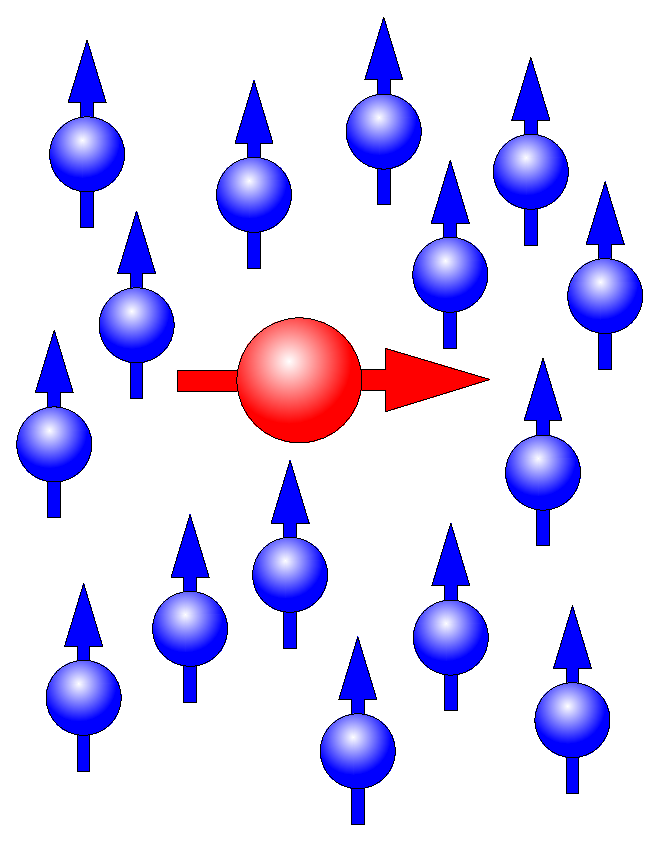
\includegraphics[width=1.5cm]{spins_sketch_pol.eps}};

  \node[inner sep=0pt, anchor=south west] at (1.82,4.625)
{  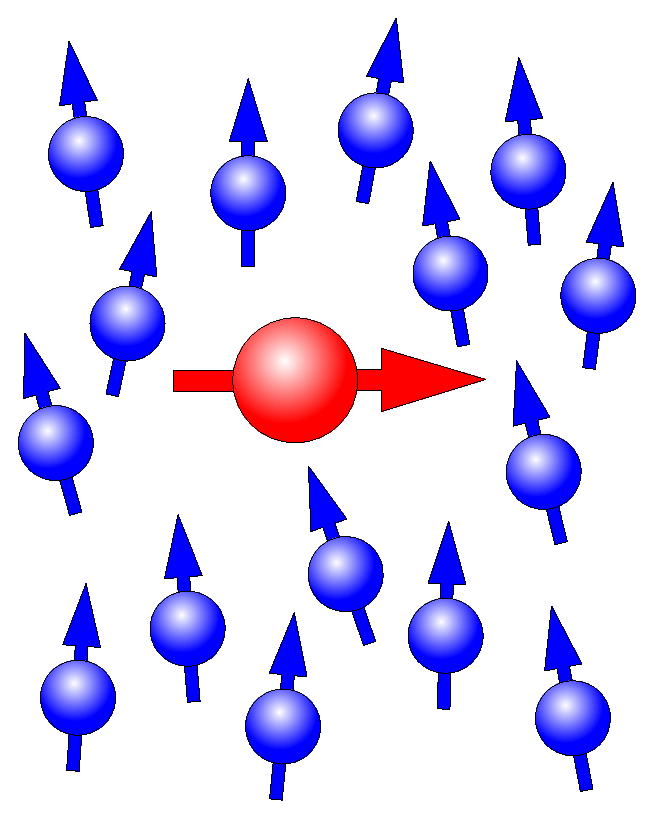
\includegraphics[width=1.5cm]{spins_sketch_part.eps}};

  \node[inner sep=0pt, anchor=south west] at (1.82,1.5)
{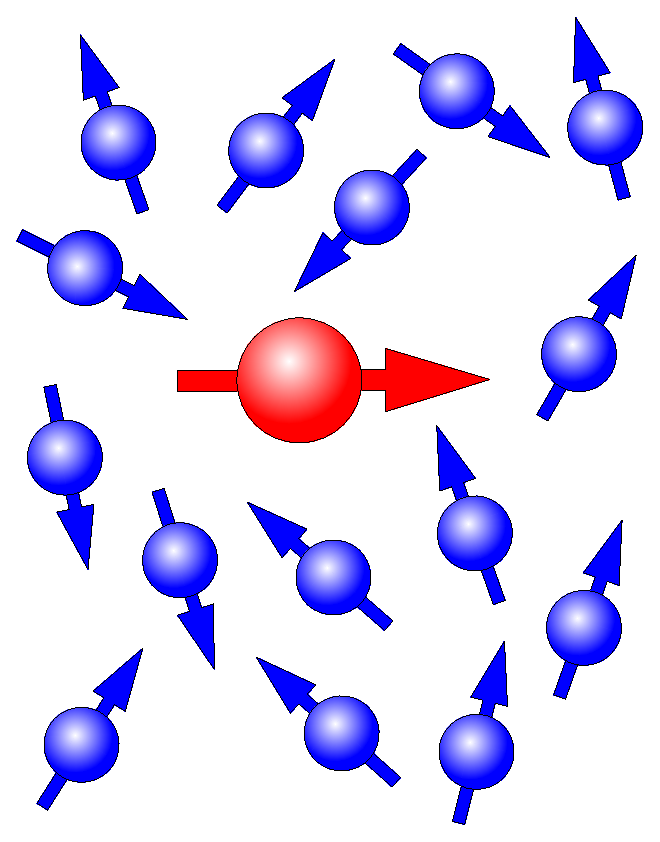
\includegraphics[width=1.5cm]{spins_sketch_unpol.eps}};

\node[inner sep=0pt, anchor=north west, scale=0.95] at (3,11.4) {
\begin{tabular}{rrrr}
$N=10:$ & $\epsilon=10^{-10}$\hspace{4mm}  &  $\epsilon=10^{-13}$ \hspace{4mm} & $\epsilon=10^{-16}$\\
$N=100:$ & $\epsilon=10^{-10}$\hspace{4mm}   &  $\epsilon=10^{-13}$ \hspace{4mm} & $\epsilon=10^{-16}$\\
$N=1000:$ &$\epsilon=10^{-10}$\hspace{4mm}   &  \multicolumn{2}{r}{analytic}
\end{tabular}
};

\end{tikzpicture}
\end{document}
